%iffalse
\let\negmedspace\undefined
\let\negthickspace\undefined
\documentclass[a4paper,12pt]{article}
\usepackage{cite}
\usepackage{amsmath,amssymb,amsfonts,amsthm}
\usepackage{algorithmic}
\usepackage{graphicx}
\usepackage{textcomp}
\usepackage{xcolor}
\usepackage{txfonts}
\usepackage{listings}
\usepackage{enumitem}
\usepackage{mathtools}
\usepackage{gensymb}
\usepackage{comment}
\usepackage[breaklinks=true]{hyperref}
\usepackage{tkz-euclide} 
\usepackage{listings}
\usepackage{gvv}                                        
%%\def\inputGnumericTable{}                                 
\usepackage[latin1]{inputenc}                                
\usepackage{color}                                            
\usepackage{array}                                            
\usepackage{longtable}                                       
\usepackage{calc}                                             
\usepackage{multirow}                                         
\usepackage{hhline}                                           
\usepackage{ifthen}                                           
\usepackage{lscape}
\usepackage{tabularx}
\usepackage{array}
\usepackage{float}
\usepackage{multicol}
\usepackage{subcaption}
\usepackage{xcolor}
\usepackage{siunitx}

\newtheorem{theorem}{Theorem}[section]
\newtheorem{problem}{Problem}
\newtheorem{proposition}{Proposition}[section]
\newtheorem{lemma}{Lemma}[section]
\newtheorem{corollary}[theorem]{Corollary}
\newtheorem{example}{Example}[section]
\newtheorem{definition}[problem]{Definition}
\newcommand{\BEQA}{\begin{eqnarray}}
\newcommand{\EEQA}{\end{eqnarray}}
\newcommand{\define}{\stackrel{\triangle}{=}}
\theoremstyle{remark}
\newtheorem{rem}{Remark}
\usepackage{graphicx}
\usepackage{geometry}
\geometry{margin=1in}
\usepackage{listings}
\lstset{
    basicstyle=\ttfamily\footnotesize, 
    breaklines=true,         % Enables line wrapping
    breakatwhitespace=true,  % Break lines only at spaces
    columns=fullflexible     % Adjusts spacing to avoid cut-off
}


% Marks the beginning of the document

\bibliographystyle{IEEEtran}
\vspace{3cm}


\title{Scientific Calculator using Arduino UNO and LCD}
\author{S. Sai Akshita - EE24BTECH11054}

\begin{document}

\maketitle

\renewcommand{\thefigure}{\theenumi}
\renewcommand{\thetable}{\theenumi}



\section{Introduction}
This document provides an in-depth explanation of the Scientific Calculator implemented using an Arduino UNO, a Liquid Crystal Display(LCD), 20+ push buttons, and other required components.

\section{Components Used}

\begin{itemize}
    \item Arduino - 1  
    \item Breadboard - 2  
    \item 16x2 LCD Display (Parallel, 16-pin, Non-I2C)
    \item USB A to USB B cable - 1  
    \item OTG adapter - 1  
    \item Jumper wires (Male-Male) - 50 to 70  
    \item Potentiometer/Resistors -$\SI{15,000}{\ohm} - 6  $and $\SI{1,000}{\ohm} - 2$ (used in this) 
    \item Push Buttons - 20 to 25  
\end{itemize}

\begin{figure}[h]
    \centering
    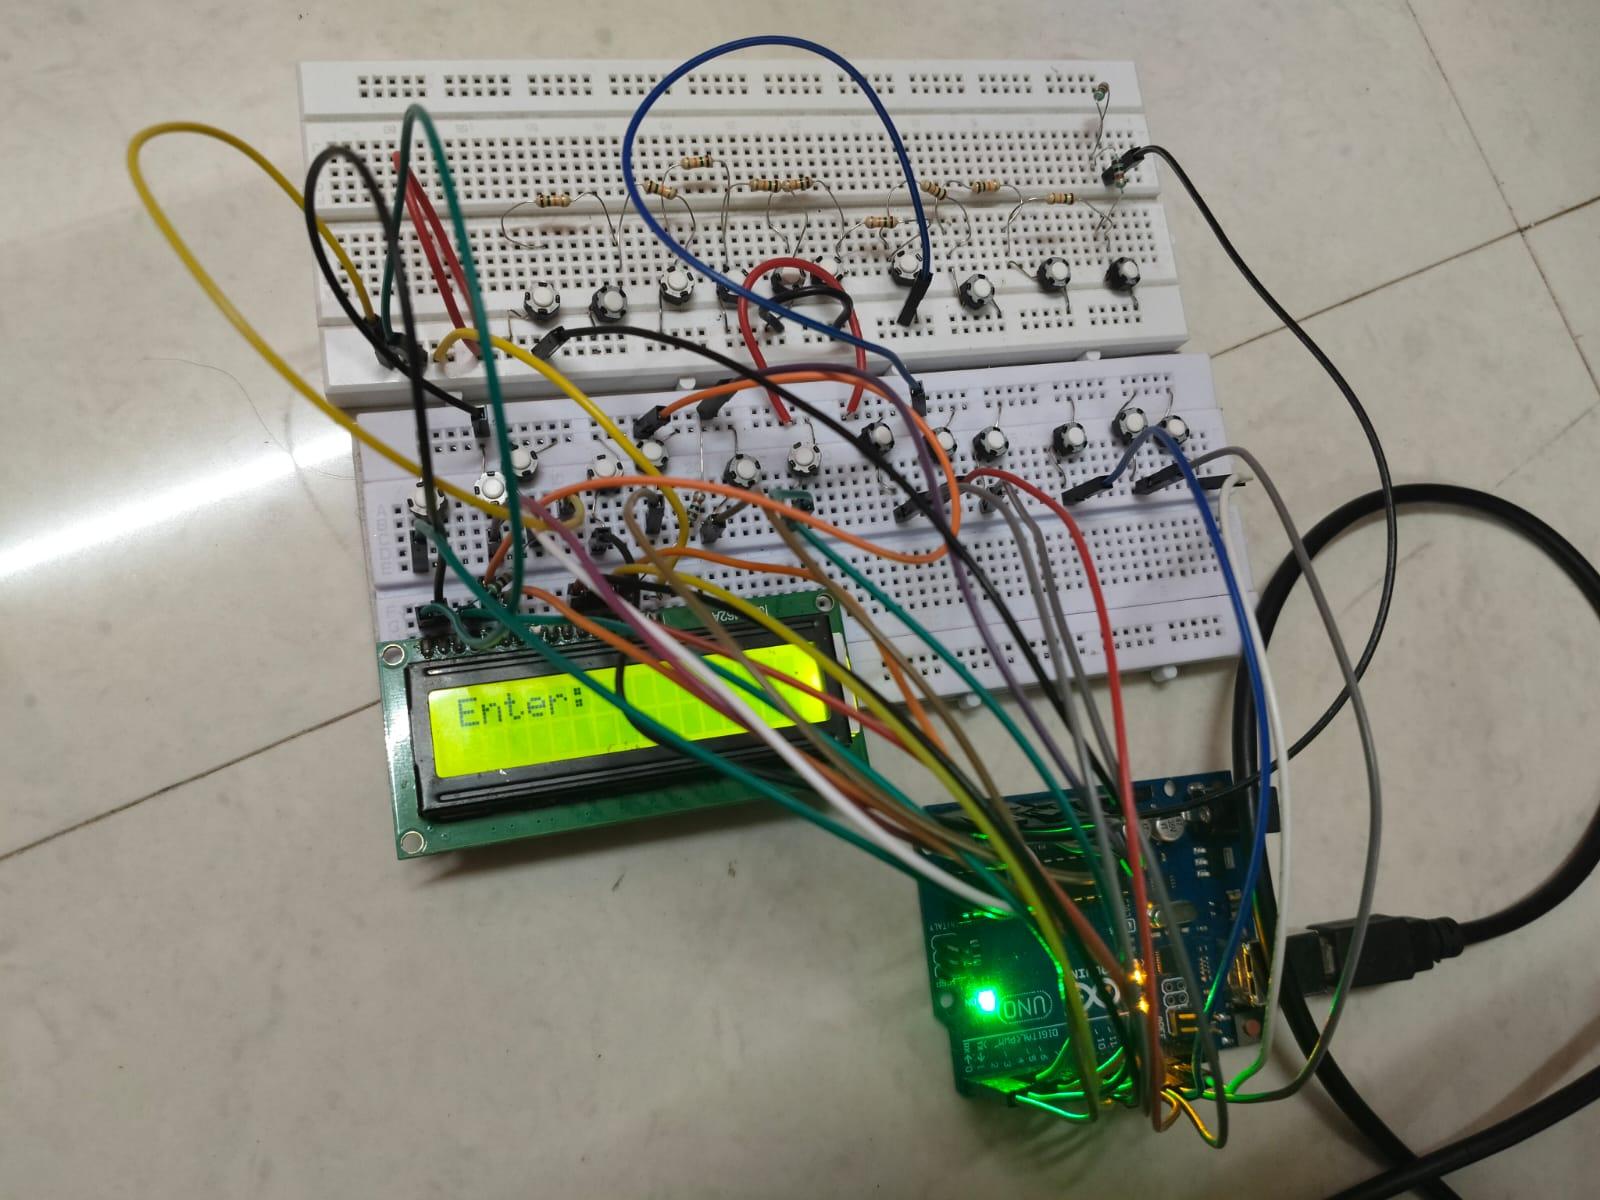
\includegraphics[width=0.8\columnwidth]{figs/fig1.jpeg} % Adjust the path
    \caption{Scientific Calculator Setup}
    \label{fig:example}
\end{figure}


\newpage
\section{Pin Configuration and Breadboard Connections}

\subsection{LCD pin configuration}
 \begin{table}[h!]
    \centering
    \begin{tabular}{|c|c|}
        \hline
        \textbf{One end of Jumper Wire}  & \textbf{Another end of Jumper Wire} \\
        \hline
          Digital pin 0 & Push button 16 \\
          Digital pin 1 & Push button 17 \\
          Digital pin 2 & LCD pin 4 \\
          Digital pin 3 & LCD pin 6 \\
          Digital pin 4 & LCD pin 11 \\
          Digital pin 5 & LCD pin 12 \\
          Digital pin 6 & LCD pin 13 \\
          Digital pin 7 & LCD pin 14 \\
          Digital pin 8 & Push button 18 \\
          Digital pin 9 & Push button 19 \\
          Digital pin 10 & Push button 20 \\
          Digital pin 11 & Push button 21 \\
          Digital pin 12 & Push button 22 \\
          Digital pin 13 & Push button 23 \\
          Analog pin A1 & Push button 15 \\
          Analog pin A2 & Push button 14 \\
          Analog pin A3 & Push button 13 \\
          Analog pin A4 & Push button 12 \\
          Analog pin A5 & Push button 11 \\
          Analog pin A0 & Push buttons 1-10 (digit buttons)\\
          LCD pin 1 & Ground \\
          LCD pin 2 & 5V \\
          LCD pin 15 & 5V via 1k $\Omega$ resistor \\
          LCD pin 16 & Ground \\
          LCD pin 3 & Ground via 1.5 k $\Omega$ resistor \\
          LCD pin 5 & Ground \\
          LCD pin 5 & All push buttons \\
          
        \hline
    \end{tabular}
\end{table}




\section{Button Connections for Scientific Calculator}

The following list outlines the button connections for the scientific calculator:

 \begin{table}[h!]
    \centering
    \begin{tabular}{|c|c|}
        \hline
        \textbf{Button number}  & \textbf{Function} \\
        \hline
           1 - 10 & Digits 0 - 9 \\
           11 & Clear \\
           12 & $\ln{(x)}$ and $\log{(x)}$ \\
           13 & Right Parenthesis \\
           14 & $\sin{(x)}$, $\cos{(x)}$, and $\tan{(x)}$ \\
           15 & $e$ and $\pi$ \\
           16 & Backspace \\
           17 & Decimal Point \\
           18 & Equal To \\
           19 & Left Parenthesis \\
           20 & Division (/)\\
           21 & Multiplications (*)\\
           22 & Subtraction(-) \\
           23 & Addition (+) \\
        \hline
    \end{tabular}
\end{table}


\newpage
\section{Power Supply Connection and Uploading Code}
The Arduino UNO is powered via USB from a mobile phone.
\begin{itemize}
    \item To compile the code and upload it into arduino UNO, run the command "make" in the directory containing .c file, header file, file containing definitions and Makefile. Then the created .hex file should be uploaded into Arduino UNO. 
\end{itemize}

\section{Circuit Working Mechanism(Analog to Digital Conversion)}
Analog-to-Digital Conversion (ADC) is a technique used to convert an analog signal into a digital value that can be processed by a microcontroller.
\subsection{ADC Fundamentals}
The ATmega328P's 10-bit ADC converts analog voltages (0-5V) to digital values (0-1023). Key characteristics include:
\begin{itemize}
    \item 10-bit resolution (1024 discrete values)
    \item 9-260$\mu$s conversion time (depending on clock prescaler)
    \item 8 multiplexed input channels (A0-A7)
\end{itemize}

\subsection{Implementation in Calculator}
\begin{itemize}
    \item \textbf{Button Matrix:}
    \begin{itemize}
        \item Digit buttons 0-9 connected via voltage divider to A0
        \item Each button produces a unique voltage level (e.g., Button1=0.5V, Button2=1.0V,...,Button9=4.5V,Button10=5V)
    \end{itemize}
    
    \item \textbf{Configuration:}
    \begin{itemize}
        \item Reference voltage: 5V
        \item Prescaler: 128 (ADC clock = 125kHz)
        \item Channel selection: ADC0 (A0 pin)
    \end{itemize}

    \item \textbf{Reading Process:}
    \begin{itemize}
        \item Single conversion initiated via ADSC bit
        \item \texttt{Conversion complete} flag (ADIF) checked for completion
        \item Result read from ADC/ADCL registers
    \end{itemize}
\end{itemize}

\subsection{Advantages of ADC for Button Inputs}
The use of ADC for button inputs offers several benefits:
\begin{itemize}
    \item \textbf{Optimized Resource Utilization:} Reduces the number of required input pins, allowing efficient microcontroller resource management.
    \item \textbf{Simplified Circuit Design:} Minimizes wiring complexity, thereby improving circuit reliability.
    \item \textbf{Accurate and Efficient Detection:} Utilizes predefined voltage thresholds to ensure precise button identification.
\end{itemize}


\subsection{Application in the Scientific Calculator}
In this project, the ADC technique is used to read multiple buttons through a single analog pin, preserving valuable digital input pins. Arithmetic operations are managed using separate digital pins, while trigonometric functions are accessed using a single button with a scrolling selection mechanism.


\section{Mechanism of Codes}

The main.c program is located in the directory named \texttt{codes}.  
Below is an overview of the essential functions used in the implementation:

\subsection{Core Mathematical Functions}
\subsubsection{Angle Conversion and Reduction}
\begin{itemize}
    \item \texttt{double reduce\_angle(double rad)}: Adjusts any angle to the range $\sbrak{0, 2\pi}$ by eliminating full rotations.  
    \item \texttt{double deg2rad(double deg)}: Converts degrees into radians using the formula $rad = deg \times \frac{\pi}{180}$.  
\end{itemize}

\subsubsection{Natural Logarithm Calculation}
\begin{itemize}
    \item \texttt{double compute\_ln(double x)}: Computes the natural logarithm by numerically integrating $\int_1^x \frac{1}{t} dt$ using the trapezoidal rule.  
\end{itemize}

\subsubsection{Numerical Methods}
\begin{itemize}
    \item \texttt{double tangent\_rk4(double radians, double h)}: Determines the tangent using the 4th-order Runge-Kutta method by solving the differential equation $\frac{dy}{dx} = -y$.
    \item \texttt{double power(double x, double n)}: Computes $x^n$ using Euler's method for the differential equation $\frac{dy}{dx} = n \cdot y$.  
\end{itemize}

\subsection{Stack Operations}
\subsubsection{Operator Stack}
\begin{itemize}
    \item \texttt{void initStack(Stack *s)}: Initializes the operator stack.  
    \item \texttt{void push(Stack *s, const char* val)}: Adds an operator to the stack.  
    \item \texttt{const char* peek(Stack *s)}: Retrieves the top element without removing it.  
\end{itemize}

\subsubsection{Number Stack}
\begin{itemize}
    \item \texttt{void initNumStack(NumStack *s)}: Initializes the number stack.  
    \item \texttt{void pushNum(NumStack *s, float val)}: Pushes a number onto the stack.  
    \item \texttt{float popNum(NumStack *s)}: Removes and returns the top number from the stack.  
\end{itemize}

\subsection{Expression Processing}
\subsubsection{Infix to Postfix Conversion}
\begin{itemize}
    \item \texttt{void infixToPostfix(const char* infix, char* postfix)}: Converts an expression from standard mathematical notation to Reverse Polish Notation using Dijkstra's shunting-yard algorithm.  
    \item This function handles:
    \begin{itemize}
        \item Parentheses grouping  
        \item Operator precedence (PEMDAS rules)  
        \item Special functions such as \texttt{trig} and \texttt{log}  
    \end{itemize}
\end{itemize}

\subsubsection{Postfix Evaluation}
\begin{itemize}
    \item \texttt{float evaluatePostfix(const char* postfix)}: Evaluates expressions written in Reverse Polish Notation using a number stack.  
    \item It supports:
    \begin{itemize}
        \item Basic arithmetic operations $(+, -, \times, \div)$  
        \item Exponentiation $(x^y)$  
        \item Trigonometric functions $(\sin, \cos, \tan)$  
        \item Logarithmic functions $(\ln, \log_{10})$  
    \end{itemize}
\end{itemize}




 

\section{Advantages of Using AVR-GCC Over C++}
Using AVR-GCC instead of C++ for implementing the digital clock provides several benefits:

\begin{itemize}
    \item \textbf{Efficiency:} AVR-GCC generates highly optimized machine code, resulting in faster execution and reduced memory usage.
    \item \textbf{Precise Timing:} Direct control over hardware registers allows for more accurate timing, crucial for maintaining a stable clock display.
    \item \textbf{Lower Overhead:} Unlike C++ with its runtime overhead, AVR-GCC offers minimal abstraction, reducing unnecessary processing load.
    \item \textbf{Fine-Grained Hardware Control:} Allows direct manipulation of registers and ports, ensuring precise control over multiplexing and display updates.
    \item \textbf{Smaller Code Size:} Since AVR-GCC avoids C++ features like classes and dynamic memory allocation, the compiled code size remains smaller.
    \item \textbf{Better Debugging:} With direct register access, debugging at the hardware level becomes more transparent compared to C++ abstractions.
\end{itemize}



\section{Precautions}
\subsection{Hardware}
\begin{itemize}
    \item \textbf{Proper Power Supply:} Ensure a stable 5V power supply to prevent voltage fluctuations that can damage components.
    \item \textbf{Secure Connections:} Use firm jumper wire connections to avoid loose connections that may cause erratic behavior.
    \item \textbf{Resistor Selection:} Choose appropriate resistors, especially for LCD contrast adjustment and button input voltage dividers.
    \item \textbf{Debouncing Buttons:} Use pull-down or pull-up resistors to prevent unintended multiple inputs due to switch bouncing.
    \item \textbf{Proper LCD Handling:} Avoid excessive pressure on the LCD screen and ensure correct pin connections to prevent damage.
    \item \textbf{Short Circuit Prevention:} Double-check wiring to avoid accidental short circuits, especially on a breadboard.
    \item \textbf{Heat Dissipation:} Ensure that components, especially the Arduino, do not overheat due to excessive current draw.
    \item \textbf{Correct Pin Assignments:} Verify connections between buttons, LCD, and microcontroller to avoid miswiring.
    \item \textbf{Static Protection:} Handle microcontroller and ICs with care to prevent static discharge damage.
    \item \textbf{Proper Grounding:} Ensure a common ground for all components to avoid floating voltage issues.
\end{itemize}
\subsection{Software}
\begin{itemize}
    \item \textbf{Efficient Code Optimization:} Keep the AVR-GCC code optimized to avoid unnecessary delays in button response.
    \item \textbf{Debounce Logic in Software:} Implement software-based debounce techniques to prevent unintended button presses.
    \item \textbf{Memory Management:} Avoid excessive memory usage to prevent crashes or unexpected behavior.
    \item \textbf{Error Handling:} Implement proper error detection and handling in calculations to prevent incorrect results.
     \item \textbf{Avoid Infinite Loops:} Ensure that the program does not get stuck in infinite loops due to misconfigured logic.
    \item \textbf{Correct Timing Functions:} Use appropriate delay functions for LCD updates without affecting button responsiveness.
    \item \textbf{Power Efficiency:} Optimize code to minimize power consumption, especially if using battery power.
    \item \textbf{Proper LCD Commands:} Use the correct initialization commands for the LCD to prevent display glitches.
    \item \textbf{Testing in Stages:} Test each component separately (LCD, buttons, arithmetic operations) before full integration.
    \item \textbf{Backup Code:} Always keep a backup of your working code before making major modifications.
\end{itemize}


\end{document}




